% \part*{Supplementary Material}
% %\begin{center}
% %	{\LARGE \textbf{Appendix}}
% %\end{center}
{
\setlength{\parskip}{-0em}
\startcontents[sections]
\printcontents[sections]{ }{1}{}
}
\clearpage

\section*{Impact Statement}
This work advances the methodological and theoretical understanding of diffusion and flow policy optimization and presents no foreseeable negative social impacts.
\section*{LLM Usage Disclosure}
We used large language models (LLMs) to aid and polish writing, such as improving clarity, grammar, and conciseness. We also used LLMs for retrieval and discovery, for example exhausting literature to identify potential missing related work. All technical content, proofs, experiments, and results are original contributions by the authors.


\section{Notation}
\label{sec:notation}
We use $\E[\cdot]$ and $\P(\cdot)$ to denote expectation and probability.
Unless otherwise specified, any expectation involving a random time $t$ is taken with respect to the uniform distribution on $[0,T]$, i.e., $t\sim \mathrm{Unif}([0,T])$.
For a time horizon $T>0$, let $\Omega=C([0,T];\mathbb R^d)$ be the trajectory space.
For any path measure $\mathbb Q$ on $\Omega$, we denote its time-$t$ marginal by $q_t$ and its conditional distribution of $X_t$ given $X_r=x_r$ by $q_{t|r}(\cdot|x_r)$.
For diffusion policies, $t=0$ denotes the action endpoint and $t=T$ denotes the noise endpoint, and the reverse denoising process is simulated from $T$ to $0$.
For flow policies, the convention is reversed: $t=0$ denotes the noise endpoint and $t=T$ denotes the action endpoint.
We write $p_t^\phi(\cdot|o)$ for the marginal distributions induced by the pretrained score model $s_\phi$ or velocity model $u_\phi$, and $p_t^h(\cdot|o)$ for the marginal distributions induced by the Doob-tilted process introduced in \cref{sec:method}.
The learned ratio model is denoted by $r_\beta(o,a)$, and in the RL setting the terminal tilt is chosen proportional to this learned ratio.
In \cref{sec:soc}, $\mathbb Q^u(\cdot|o)$ denotes the controlled path measure induced by the control $u_t(\cdot,o)$, and $q_t^u(\cdot|o)$ denotes its time-$t$ marginal distribution.
When no ambiguity arises, we use the same lowercase notation for a probability distribution and its density.
Unless otherwise specified, the state distribution used in expectations is assumed to have full support on $\mathcal S$.
We write $\mathbb R_+ := (0,\infty)$.
We say the model class $\{s_\theta:\theta\in\Theta\}$ is realizable for the Doob drift if there exists $\theta^\star\in\Theta$ such that
$s_{\theta^\star}(x,t,o)=\nabla_x\log h_t(x,o)$
for every $x\in\mathcal A$, $t\in[0,T]$, and $o \in\mathcal S$.


\section{Related Works}
\label{sec:related_works}


\paragraph{Diffusion Model and Diffusion Policy.}
Diffusion models \cite{sohldickstein2015deep,ho2020denoising} are probabilistic generative models that progressively transform noise into samples from a target distribution. They are closely connected to score-based generative modeling \cite{song2019generative,song2021scorebased}, which offers a complementary view based on learning the gradient field of the data distribution and unifies diffusion-based generation under the stochastic differential equation framework. Owing to their strong expressiveness for complex, high-dimensional, and multimodal distributions, diffusion models have become increasingly attractive for control and decision-making. In particular, diffusion policies parameterize action distributions with diffusion models and generate actions through iterative denoising, yielding richer policy classes than standard unimodal Gaussian actors. Prior work has shown strong empirical performance of diffusion policies in visuomotor control and robotic manipulation \cite{chi2025diffusion}, as well as in goal-conditioned imitation learning and language- or play-conditioned skill learning \cite{reuss2023goalconditionedimitationlearningusing,chen2023playfusionskillacquisitiondiffusion}.

More recently, diffusion policies have been extended to online reinforcement learning. Methods such as DPPO and related diffusion-policy RL approaches show that diffusion-based policy classes can be optimized effectively beyond pure imitation learning \cite{ren2024diffusion,ma2025efficient}. Our work builds on this line of research, but focuses on RL fine-tuning of diffusion policies in the likelihood-intractable setting.

We compare against five recent diffusion-policy RL baselines: DIPO \cite{yang2023policyrepresentationdiffusionprobability}, DPPO \cite{ren2024diffusion}, DPMD \cite{ma2025efficient}, DACER \cite{wang2024diffusionactorcriticentropyregulator}, and SDAC \cite{ma2025efficient}. These baselines cover both off-policy and on-policy diffusion RL methods: DIPO, DPMD, DACER, and SDAC are off-policy, whereas DPPO is on-policy. DIPO adopts a two-stage strategy that first updates state-action particles using value gradients and then distills them into a diffusion policy. 
DPPO formulates policy optimization over a diffusion-augmented MDP and applies Proximal Policy Optimization to the resulting process. 
DPMD studies efficient online RL for diffusion policies through a policy-mirror-descent-style update with an analytic target ratio. DACER directly backpropagates value gradients through the reverse diffusion process and introduces entropy regularization to improve exploration. SDAC extends diffusion-policy optimization to the soft-actor-critic regime with an analytic-ratio-based update. 

Our work generalizes the analytic-ratio ideas underlying DPMD and SDAC into a unified likelihood-free framework, extending them from diffusion policies to flow matching policies and to a broader class of policy optimization methods, including PPO \cite{schulman2017proximal} and GRPO \cite{shao2024deepseekmath}.

\paragraph{Flow Matching Model and Flow Policy.}
Flow matching \cite{lipman2022flow,liu2022flow} provides an alternative to diffusion models by learning a deterministic ODE transport between a noise prior and the data distribution. Compared to diffusion models, flow matching avoids simulating stochastic dynamics during training and offers faster sampling through fewer integration steps. These properties have made flow matching models increasingly popular in decision-making applications. $\pi_0$ \cite{black2024pi} and its successor $\pi_{0.5}^*$ \cite{intelligence2025pi} adopt flow matching as the generative backbone of vision-language-action models for general robot manipulation, demonstrating that flow policies can scale to diverse real-world tasks. However, the likelihood of a flow policy is as intractable as that of a diffusion policy, since it requires solving an ODE and computing the associated log-determinant of the Jacobian. This intractability poses the same challenge for online RL fine-tuning: standard policy gradient methods that rely on likelihood ratios cannot be directly applied. Flow Q-Learning \cite{park2025flow} is an early attempt that sidesteps this issue by using Q-function guidance to steer the flow sampling process, analogous to Q-guided diffusion methods. For policy gradient approaches, several workarounds have been proposed. FPO \cite{mcallister2025flow} is a PPO-style method that replaces explicit policy ratios with an implicit surrogate derived from the flow matching training loss, avoiding likelihood computation entirely. ReinFlow \cite{zhang2025reinflow} converts a deterministic flow policy into a stochastic short-horizon Markov process via learned noise injection, enabling tractable stepwise likelihood computation for policy gradient updates. Flow-SDE \cite{chen2025pirl} instead replaces the deterministic flow ODE with an analytically constructed stochastic differential equation, yielding explicit transition probabilities suitable for policy gradient estimation. All these methods require some form of likelihood evaluation or surrogate at the denoising steps; in contrast, our approach bypasses this requirement entirely by learning a lightweight ratio network that directly estimates the probability ratio needed for policy optimization.








\section{\texorpdfstring{Proof of \cref{lem:algo_correctness}}{Proof of Theorem \ref{lem:algo_correctness}}}
\label{sec:proof_corr}
\begin{lemma}[\cref{lem:algo_correctness} Restated: Doob's $h$-Transform]
Fix a state $o \in\mathcal{S}$.
Let $(X_t)_{t\in[0,T]}$ follow the reverse-time denoising SDE \eqref{eq:reverse_sde} with $\nabla_x \log p_t(x|o)$ replaced by its estimator $s_\phi(x,t,o)$, inducing conditional marginals 
$\{p_t^\phi(\cdot|o)\}_{t\in[0,T]}$.
Let $h_0(\cdot,o):\mathcal{A}\to\R_+$ be a positive integrable function.
Let $h(\cdot,o,\cdot):\mathcal{A}\times[0,T]\to \R_+$ be the associated Doob $h$-function, denoted by $h_t(x,o)$, defined as
\begin{align*}
    h_t(x,o)
    =
    \E \big[h_0(X_0,o)| X_t=x,o\big],
\end{align*}
where the conditional expectation is taken under the original (untilted) denoising process induced by $s_\phi$.
The Doob $h$-transformed denoising process starts from
\[
    X_T^h \sim p_T^h(\cdot|o),
    \qquad
    p_T^h(x|o)
    :=
    \frac{
        p_T^\phi(x|o) h_T(x,o)
    }{
        \E_{X_0\sim p_0^{\phi}(\cdot|o)}[h_0(X_0,o)]
    },
\]
and evolves backward from $T$ to $0$ according to
\begin{align*}
    \dd X_t^{h}
    =
    \Big[
        f(X_t^{h},t)
        -\sigma_t^2 s_\phi(X_t^{h},t,o)
        -\sigma_t^2 \nabla_x \log h_t(X_t^{h},o)
    \Big]\dd t
    +\sigma_t\dd W_t.
\end{align*}
Then its conditional marginals satisfy
\begin{align*}
    p_t^{h}(x|o)
    =
    \frac{
        p_t^\phi(x|o)h_t(x,o)
    }{
        \E_{X_0\sim p_0^{\phi}(\cdot|o)}[h_0(X_0,o)]
    },
    \quad t\in[0,T].
\end{align*}
In particular, taking $h_0(x,o)=r_\beta(o,x)$ yields
\[
    p_0^h(x|o)
    \propto
    p_0^{\phi}(x|o)r_\beta(o,x).
\]
Since $p_0^{\phi}(\cdot|o)=\pi_{\mathrm{old}}(\cdot|o)$, the time-$0$ policy induced by the tilted denoising process satisfies
\begin{align*}
    \pi(a|o)
    \propto
    r_\beta(o,a)\pi_{\mathrm{old}}(a|o).
\end{align*}
\end{lemma}



\begin{proof}
Conditioning on the fixed state $o$, the original denoising process is a reverse-time Markov process
with marginals $\{p_t^\phi(\cdot|o)\}_{t\in[0,T]}$ and time-$0$ tilting function $h_0(\cdot,o)$.
By the continuous-time Doob $h$-transform for reverse-time diffusion processes
\cite[Proposition~2]{nguyen2025h}, the transformed process evolves backward from $T$ to $0$ according to
\begin{align*}
    \dd X_t^{h}
    =
    \Big[
        f(X_t^{h},t)
        -\sigma_t^2 s_\phi(X_t^{h},t,o)
        -\sigma_t^2 \nabla_x \log h_t(X_t^{h},o)
    \Big]\dd t
    +\sigma_t\dd W_t.
\end{align*}
which is exactly \eqref{eq:new_process}.
It remains to identify its marginals. By the reverse-time Doob bridge marginal identity
\cite[Proposition~1]{nguyen2025h}, also see \cite[Section~3.2]{zhu2026training}, if the transformed process starts from
\[
    p_T^h(x|o)
    =
    \frac{
        p_T^\phi(x|o)h_T(x,o)
    }{
        \E_{X_0\sim p_0^\phi(\cdot|o)}[h_0(X_0,o)]
    },
\]
then, for every $t\in[0,T]$,
\[
    p_t^h(x|o)
    =
    \frac{
        p_t^\phi(x|o)h_t(x,o)
    }{
        \E_{X_0\sim p_0^\phi(\cdot|o)}[h_0(X_0,o)]
    }.
\]
This proves \eqref{eq:p_t^h}.
Taking $t=0$ gives
\[
    p_0^h(a|o)
    =
    \frac{
        p_0^\phi(a|o)h_0(a,o)
    }{
        \E_{X_0\sim p_0^\phi(\cdot|o)}[h_0(X_0,o)]
    }.
\]
In particular, with $h_0(a,o)=r_\beta(o,a)$,
\[
    p_0^h(a|o)
    \propto
    p_0^\phi(a|o)r_\beta(o,a).
\]
Since $p_0^\phi(\cdot|o)=\pi_{\mathrm{old}}(\cdot|o)$, the time-$0$ policy induced by the tilted
denoising process satisfies
\[
    \pi(a|o)
    \propto
    r_\beta(o,a)\pi_{\mathrm{old}}(a|o).
\]
\end{proof}



\section{\texorpdfstring{Proof of \cref{thm:grad_equi_diff}}{Proof of Theorem \ref{thm:grad_equi_diff}}}
\label{sec:proof_grad_equi}

\begin{theorem}[\cref{thm:grad_equi_diff} Restated: Gradient Equivalence for Diffusion]
\label{thm:grad_equi_re}
    Let $\mathcal{L}_{\mathrm{DM}}$ and $\mathcal{L}_{\mathrm{CDM}}$ be defined in \eqref{eq:def_DM} and \eqref{eq:def_cDM}, respectively.
Fix state $o \in\mathcal S$, define normalizing constant
$Z_{\beta}(o) := \E_{X_0 \sim p_0^\phi(\cdot|o)}\big[r_\beta(o,X_0)\big]$and 
\begin{align*}
    \ell_{\mathrm{DM}}(\theta,o)
    &:=
    \E_{t,X_t\sim p_t^h(\cdot|o)}
    \left[
        \|
        \nabla_x\log h_t(X_t,o)-s_\theta(X_t,t,o)
        \|_2^2
    \right],
    \\
    \ell_{\mathrm{CDM}}(\theta,o)
    &:=
    \E_{t,X_t\sim p_t^\phi(\cdot|o),X_0\sim p_{0|t}^\phi(\cdot|X_t,o)}
    \left[
        r_\beta(o,X_0)
        \|
        \nabla_x\log p_{0|t}^\phi(X_0|X_t,o)
        -
        s_\theta(X_t,t,o)
        \|_2^2
    \right].
\end{align*}
Then their gradients satisfy
\begin{align*}
    \nabla_\theta \ell_{\mathrm{CDM}}(\theta,o)
    =
    Z_{\beta}(o) \cdot \nabla_\theta \ell_{\mathrm{DM}}(\theta,o).
\end{align*}
% If the model class $\{s_\theta:\theta\in\Theta\}$ is realizable and the minimum of $L_{\mathrm{CDM}}$ is attained, then any minimizer $s_\theta^\star$ of $L_{\mathrm{CDM}}$ satisfies
% $s_\theta^\star(x,t,o)
% =\nabla_x\log h_t(x,o)$
% for every $x\in\mathcal A$, $t\in[0,T]$, and $o \in\mathcal S$.
\end{theorem}

\begin{proof}
For notational simplicity, we first present the proof in the unconditional setting.
That is, the conditioning variable $o$ is fixed and omitted from the notation.
The conditional statement follows by applying the same argument pointwise for each $o \in\mathcal S$, with
$p_t(\cdot)$, $p_t^h(\cdot)$, $p_{0|t}(\cdot|\cdot)$, $h_t(\cdot)$, and $r_\beta(\cdot)$ replaced by
$p_t^\phi(\cdot|o)$, $p_t^h(\cdot|o)$, $p_{0|t}^\phi(\cdot|\cdot,o)$, $h_t(\cdot,o)$, and $r_\beta(o,\cdot)$, respectively.
We now expand the unconditional drift matching loss.
\begin{align}
\label{eq:derivation_all_sm}
    \ell_{\text{DM}}(\theta)
    = & ~ \E_{t, X_t \sim p_t^h}
    [\| \nabla \log h_t(X_t)
    - s_\theta(X_t,t)\|_2^2] \\
    =\frac1T & ~ \int_0^T \int_{\R^d}
    \left[\|\nabla_x \log h_t(x)\|_2^2 + \|s_\theta(x,t)\|_2^2 - 2s_\theta(x,t)^\top \nabla_x \log h_t(x)\right]
    p_t^h(x)
    \dd x \dd t \nonumber\\
    =\frac1T & ~ \int_0^T \int_{\R^d} \left[\|s_\theta
    (x,t)\|_2^2 - 2
    s_\theta(x,t)^\top \nabla_x \log h_t(x)\right]
    p_t^h(x) 
    \dd x \dd t + C_1,
\end{align}
where $C_1 := \frac1T \int_0^T \int_{\R^d}
\|\nabla \log h_t(x)\|_2^2 
p_t^h(x) \dd x \dd t~$ is independent to $\theta$.
For the first term, 
\begin{align}
    & ~\frac1T  \int_0^T \int_{\R^d} \|s_\theta
    (x,t)\|_2^2 
    p_t^h(x)  
    \dd x \dd t \nonumber\\
    = & ~ \frac{1}{Z_{\beta}(o)T} \int_0^T \int_{\R^d} \|s_\theta
    (x,t)\|_2^2 \cdot
    h_t(x) p_t(x) 
    \dd x \dd t \annot{By $p_t^h(x) \propto p_t(x) h_t(x)$} \\
    = & ~ \frac{1}{Z_{\beta}(o)} \E_{t,X_t \sim p_t}[\|s_\theta
    (X_t,t)\|_2^2 h(X_t,t)] \nonumber\\
    = & ~ \frac{1}{Z_{\beta}(o)} \E_{t,X_t \sim p_t}[\|s_\theta
    (X_t,t)\|_2^2 \E_{X_0 \sim p_{0|t}}[r_\beta(X_0)|X_t]] \annot{By $ h(X_t,t)=
    \E[h(X_0,0)|X_t]$ follows from \eqref{eq:solution_exp}}\\
    = & ~ \frac{1}{Z_{\beta}(o)} \E_{t,X_t \sim p_t, X_0 \sim p_{0|t}}[\|s_\theta
    (X_t,t)\|_2^2 \cdot r_\beta(X_0)],
    \label{eq:derivation_all_first}
\end{align}
where $Z_{\beta}(o) = \int_{\R^d} p_t(x) h_t(x) \dd x = \E_{X_t \sim p_t}[h(X_t,t)] = \E_{X_0 \sim p_0}[r_\beta(X_0)]$ is the normalizing constant and the last equation follows from \eqref{eq:solution_exp} and tower property.  
Next we focus on the second term.
We show that
\begin{align*}
    & ~ \frac1T \int_0^T \int_{\R^d}
    s_\theta(x,t)^\top \nabla_x \log h_t(x)
    p_t^h(x)
    \dd x \dd t \\
    = & ~ \frac1T \int_0^T \int_{\R^d}
    s_\theta(x,t)^\top \frac{\nabla_x h_t(x)}{h_t(x)}
    p_t^h(x) 
    \dd x \dd t \annot{By $\nabla_x \log h_t(x) = \nabla_x h_t(x)/ h_t(x)$}\\
    = & ~ \frac{1}{Z_{\beta}(o)T=}\int_0^T \int_{\R^d}
    s_\theta(x,t)^\top \frac{\nabla_x h_t(x)}{h_t(x)}
    p_t(x) h_t(x) 
    \dd x \dd t \annot{By $p_t^h(x) \propto p_t(x) h_t(x)$}\\
    = & ~ \frac{1}{Z_{\beta}(o)T}\int_0^T \int_{\R^d}
    s_\theta(x,t)^\top 
    \nabla_x h_t(x)
    p_t(x)  
    \dd x \dd t.
\end{align*}
Next, we consider conditioning by recalling $h_t(x) = \int_{\R^d} r_\beta(z) p_{0|t}(z|x) \dd z$ follows from \eqref{eq:solution_exp}.
\begin{align}
\label{eq:derivation_second_t}
    & ~ \frac1T\int_0^T \int_{\R^d}
    s_\theta(x,t)^\top \nabla_x  \log h_t(x)
    p_t^h(x)
    \dd x \dd t \nonumber\\
    = & ~ \frac{1}{Z_{\beta}(o)T}\int_0^T \int_{\R^d}
    s_\theta(x,t)^\top 
    \left(\int_{\R^d} r_\beta(z) \nabla_{x} p_{0|t}(z|x) \dd z \right)
    p_t(x)  
    \dd x \dd t \nonumber\\
    = & ~ \frac{1}{Z_{\beta}(o)T}\int_0^T \int_{\R^d}
    s_\theta(x,t)^\top 
    \left(\int_{\R^d} r_\beta(z) 
    \frac{\nabla_{x} p_{0|t}(z|x)}{p_{0|t}(z|x)} \cdot p_{0|t}(z|x) \dd z \right)
    p_t(x)  
    \dd x \dd t \nonumber\\
    = & ~ \frac{1}{Z_{\beta}(o)T}\int_0^T \int_{\R^d}
    s_\theta(x,t)^\top 
    \int_{\R^d} r_\beta(z) 
    \nabla_x \log p_{0|t}(z|x) \cdot 
    p_{0|t}(z|x) p_t(x)  
    \dd z \dd x \dd t \nonumber \\
    = & ~ \frac{1}{Z_{\beta}(o)}
    \E_{t, X_t \sim p_t, X_0 \sim p_{0|t}}[r_\beta(X_0) \cdot s_\theta(X_t,t)^\top \nabla_{X_t} \log p_{0|t}(X_0|X_t)].
\end{align}
Substituting \eqref{eq:derivation_all_first} and \eqref{eq:derivation_second_t} back to \eqref{eq:derivation_all_sm}, we show that 
\begin{align*}
    \ell_{\text{DM}}(\theta)
    = \frac{1}{Z_{\beta}}
    \E_{t, X_t \sim p_t, X_0 \sim p_{0|t}}[ r_\beta(X_0) \cdot \left(\|s_\theta(X_t,t)\|_2^2 -2 s_\theta(X_t,t)^\top \nabla_{X_t} \log p_{0|t}(X_0|X_t) \right)] + C_1.
\end{align*}
By the definition of Conditional Drift Matching loss, 
we have
\begin{align*}
    & ~ \ell_{\text{CDM}}(\theta) \\
    =  & ~ \E_{t, X_t \sim p_t, X_0 \sim p_{0|t}}[r_\beta(X_0) \cdot \|\nabla_{X_t} \log p_{0|t}(X_0|X_t) - s_\theta(X_t,t) \|_2^2] \annot{By definition \eqref{eq:def_cDM}}\\
    = & ~ \E_{t, X_t \sim p_t, X_0 \sim p_{0|t}}[ r_\beta(X_0) \cdot \left(\|s_\theta
    (X_t,t)\|_2^2 -2 s_\theta(X_t,t)^\top \nabla_{X_t} \log p_{0|t}(X_0|X_t) \right)] + C_2,
\end{align*}
where $C_2 := \E_{t, X_t \sim p_t, X_0 \sim p_{0|t}}[ \| \nabla_{X_t} \log p_{0|t}(X_0|X_t)\|_2^2 \cdot r_\beta(X_0)]$ is independent to $\theta$.
Therefore, 
\begin{align*}
    \ell_{\text{CDM}}(\theta)
    = Z_{\beta}(o)(\ell_{\text{DM}}(\theta)-C_1)+C_2.
\end{align*}
Taking gradients with respect to $\theta$ gives
\begin{align*}
    \nabla_\theta  \ell_{\mathrm{CDM}}(\theta)
    =
    Z_{\beta}(o) \nabla_\theta \ell_{\mathrm{DM}}(\theta),
\end{align*}
since $C_1$ and $C_2$ are independent of $\theta$.

% Returning to the conditional setting, the above derivation gives, for each fixed $o \in\mathcal S$,
% \begin{align*}
%     \ell_{\mathrm{CDM}}(\theta,o)
%     =
%     Z_{\beta}(o)
%     [
%         \ell_{\mathrm{DM}}(\theta,o)-C_1(s)
%     ]
%     +
%     C_2(s),
% \end{align*}
% where $C_1(s)$ and $C_2(s)$ are independent of $\theta$.
% Taking the expectation over $s$ gives
% \begin{align*}
%     \mathcal{L}_{\mathrm{CDM}}(\theta)
%     =
%     \E_s
%     [
%         Z_{\beta}(o)\ell_{\mathrm{DM}}(\theta,o)
%     ]
%     +
%     C,
% \end{align*}
% where $C:=\E_s[C_2(s)-Z_{\beta}(o)C_1(s)]$ is independent of $\theta$.

% It remains to identify the minimizer under realizability. By the realizability assumption, there exists $\theta^\star\in\Theta$ such that
% \begin{align*}
%     s_{\theta^\star}(x,t,o)
%     =
%     \nabla_x\log h_t(x,o)
% \end{align*}
% for every $x\in\mathcal A$, $t\in[0,T]$, and $o \in\mathcal S$.
% Hence $\ell_{\mathrm{DM}}(\theta^\star,o)=0$ for every $s$.
% Since $\ell_{\mathrm{DM}}(\theta,o)\ge 0$ and $Z_{\beta}(o)>0$, the state-reweighted objective
% \begin{align*}
%     \E_s
%     [
%         Z_{\beta}(o)\ell_{\mathrm{DM}}(\theta,o)
%     ]
% \end{align*}
% is minimized only when $\ell_{\mathrm{DM}}(\theta,o)=0$ for every $s$ 
% \footnote{Throughout this work, the state distribution used in the expectation is assumed to have full support on $\mathcal S$.}.
% Therefore, any minimizer $s_\theta^\star$ of $L_{\mathrm{CDM}}$ satisfies
% \begin{align*}
%     s_\theta^\star(x,t,o)
%     =
%     \nabla_x\log h_t(x,o)
% \end{align*}
% for every $x\in\mathcal A$, $t\in[0,T]$, and $o \in\mathcal S$.
% This completes the proof.
\end{proof}










\section{\texorpdfstring{Proof of \cref{thm:grad_equi_fm}}{Proof of Theorem \ref{thm:grad_equi_fm}}}
\label{sec:proof_grad_equi_fm}
\begin{theorem}[\cref{thm:grad_equi_fm} Restated: Gradient Equivalence for Flow]
Let $\mathcal{L}_{\mathrm{DM}}$ and $\mathcal{L}_{\mathrm{CDM}}$ be defined in \eqref{eq:def_DM_fm} and \eqref{eq:def_cDM_fm}, respectively.
Fix $o \in\mathcal S$, define normalizing constant
$Z_{\beta}(o) := \E_{X_T \sim p_T^\phi(\cdot|o)}\big[r_\beta(o,X_T)\big]$and 
\begin{align*}
    \ell_{\mathrm{DM}}(\theta,o)
    &:=
    \E_{t, X_t \sim p_t^\beta(\cdot|o)}
    \Big[
        \big\|
            u^\beta(X_t,t,o)
            - u_\theta(X_t,t,o)
        \big\|_2^2
    \Big].
    \\
    \ell_{\mathrm{CDM}}(\theta,o)
    &:=
    \E_{t, X_t \sim p_t^\phi, X_T \sim p_{T| t}^\phi}
    \Big[
        r_\beta(o,X_T)
        \big\|
            u^\beta(X_t| X_T,t,o)
            - u_\theta(X_t,t,o)
        \big\|_2^2
    \Big].
\end{align*}
Then their gradients satisfy
\begin{align*}
    \nabla_\theta \ell_{\mathrm{CDM}}(\theta,o)
    =
    Z_{\beta}(o) \cdot \nabla_\theta \ell_{\mathrm{DM}}(\theta,o).
\end{align*}
\end{theorem}
\begin{proof}
For each \(t\in[0,T]\), define $\bar r_t(x,o)$
\[
\bar r_t(x,o)
:=
\E_{X_T\sim p_{T|t}^\phi(\cdot|x,o)}
\big[
r_\beta(o,X_T)
\big].
\]
By the ratio-tilted construction of the flow path, the marginal
\(p_t^\beta(\cdot|o)\) satisfies
\begin{align}
Z_{\beta}(o)p_t^\beta(x|o)
=
p_t^\phi(x|o)\bar r_t(x,o).
\label{eq:fm-marginal-reweighting}
\end{align}
Consequently, for any fixed \(t\in[0,T]\) and any integrable test
function \(\psi\), we have
\begin{align}
\begin{aligned}
&Z_{\beta}(o)
\E_{X_t\sim p_t^\beta(\cdot|o)}
\big[
\psi(X_t)
\big]
\\
&=
Z_{\beta}(o)\int \psi(x)p_t^\beta(x|o)\dd x
\\
&=
\int \psi(x)p_t^\phi(x|o)\bar r_t(x,o)\dd x
\\
&=
\int \psi(x)p_t^\phi(x|o)
\left[
\int r_\beta(o,a)p_{T|t}^\phi(a|x,o)\dd a
\right]dx
\\
&=
\int\!\!\int
r_\beta(o,a)\psi(x)
p_{T|t}^\phi(a|x,o)p_t^\phi(x|o)
\dd a \dd x
\\
&=
\E_{\substack{
X_t\sim p_t^\phi(\cdot|o),\\
X_T\sim p_{T|t}^\phi(\cdot|X_t,o)
}}
\big[
r_\beta(o,X_T)\psi(X_t)
\big].
\end{aligned}
\label{eq:fm3}    
\end{align}

To derive the velocity reweighting identity, we use the marginalization
identity for the tilted flow:
\[
u^\beta(x,t,o)
=
\E_{X_T\sim p_{T|t}^\beta(\cdot|x,o)}
\big[
u^\beta(x|X_T,t,o)
\big].
\]
Multiplying both sides by \(p_t^\beta(x|o)\), we obtain
\[
\begin{aligned}
p_t^\beta(x|o)u^\beta(x,t,o)
&=
p_t^\beta(x|o)
\int
u^\beta(x|a,t,o)
p_{T|t}^\beta(a|x,o)\dd a
\\
&=
\int
u^\beta(x|a,t,o)
p_t^\beta(x|o)
p_{T|t}^\beta(a|x,o)\dd a .
\end{aligned}
\]
Using the ratio-tilted joint relation
\[
p_t^\beta(x|o)p_{T|t}^\beta(a|x,o)
=
\frac{r_\beta(o,a)}{Z_{\beta}(o)}
p_t^\phi(x|o)p_{T|t}^\phi(a|x,o),
\]
we get
\[
\begin{aligned}
p_t^\beta(x|o)u^\beta(x,t,o)
&=
\frac{1}{Z_{\beta}(o)}
p_t^\phi(x|o)
\int
r_\beta(o,a)
u^\beta(x|a,t,o)
p_{T|t}^\phi(a|x,o)\dd a
\\
&=
\frac{1}{Z_{\beta}(o)}
p_t^\phi(x|o)
\E_{X_T\sim p_{T|t}^\phi(\cdot|x,o)}
\big[
r_\beta(o,X_T)u^\beta(x|X_T,t,o)
\big].
\end{aligned}
\]
Equivalently,
\begin{align}
Z_{\beta}(o)p_t^\beta(x|o)u^\beta(x,t,o)
=
p_t^\phi(x|o)
\E_{X_T\sim p_{T|t}^\phi(\cdot|x,o)}
\big[
r_\beta(o,X_T)u^\beta(x|X_T,t,o)
\big].
\label{eq:fm2}
\end{align}
Now we convert \eqref{eq:fm2} into a test-function
identity. For any integrable test function \(h\), multiply
both sides of \eqref{eq:fm2} by
\(h(x,t,o)^\top\) and integrate over \(x\). This gives

\begin{align}
&Z_{\beta}(o)
\E_{X_t\sim p_t^\beta(\cdot|o)}
\big[
h(X_t,t,o)^\top u^\beta(X_t,t,o)
\big]
\notag \\
&=
Z_{\beta}(o)\int
h(x,t,o)^\top u^\beta(x,t,o)p_t^\beta(x|o)\dd x
\notag \\
&=
\int
h(x,t,o)^\top
p_t^\phi(x|o)
\E_{X_T\sim p_{T|t}^\phi(\cdot|x,o)}
\big[
r_\beta(o,X_T)u^\beta(x|X_T,t,o)
\big]
\dd x
\notag \\
&=
\int\!\!\int
r_\beta(o,a)
h(x,t,o)^\top u^\beta(x|a,t,o)
p_{T|t}^\phi(a|x,o)p_t^\phi(x|o)
\dd a\dd x
\notag \\
&=
\E_{\substack{
X_t\sim p_t^\phi(\cdot|o),\\
X_T\sim p_{T|t}^\phi(\cdot|X_t,o)
}}
\big[
r_\beta(o,X_T)
h(X_t,t,o)^\top u^\beta(X_t|X_T,t,o)
\big].\label{eq:fm1}
\end{align}

We now prove the gradient identity directly. Under the usual regularity
conditions allowing differentiation under the expectation,
\[
\begin{aligned}
\nabla_\theta \ell_{\mathrm{DM}}(\theta,o)
&=
2\E_{t,\,X_t\sim p_t^\beta(\cdot|o)}
\Big[
\big(\nabla_\theta u_\theta(X_t,t,o)\big)^\top
\big(
u_\theta(X_t,t,o)-u^\beta(X_t,t,o)
\big)
\Big].
\end{aligned}
\]
Multiplying both sides by \(Z_{\beta}(o)\), and applying
\eqref{eq:fm3} componentwise to
\[
\psi(x)
=
\big(\nabla_\theta u_\theta(x,t,o)\big)^\top
u_\theta(x,t,o),
\]
together with \eqref{eq:fm1} with
\(h=\nabla_\theta u_\theta\), gives
\begin{align}
&Z_{\beta}(o)\nabla_\theta \ell_{\mathrm{DM}}(\theta,o)\notag
\\
&=
2\E_{\substack{
t\sim U[0,T],\,
X_t\sim p_t^\phi(\cdot|o),\\
X_T\sim p_{T|t}^\phi(\cdot|X_t,o)
}}
\Big[
r_\beta(o,X_T)
\big(\nabla_\theta u_\theta(X_t,t,o)\big)^\top
\big(
u_\theta(X_t,t,o)-u^\beta(X_t|X_T,t,o)
\big)
\Big].
\label{eq:fm-dm-gradient-reweighted}
\end{align}

On the other hand, differentiating \(\ell_{\mathrm{CDM}}(\theta,o)\)
directly gives
\begin{align}
&\nabla_\theta \ell_{\mathrm{CDM}}(\theta,o)\notag \\
&=
2\E_{\substack{
t\sim U[0,T],\,
X_t\sim p_t^\phi(\cdot|o),\\
X_T\sim p_{T|t}^\phi(\cdot|X_t,o)
}}
\Big[
r_\beta(o,X_T)
\big(\nabla_\theta u_\theta(X_t,t,o)\big)^\top
\big(
u_\theta(X_t,t,o)-u^\beta(X_t|X_T,t,o)
\big)
\Big].\label{eq:fm-cdm-gradient}
\end{align}

Comparing \eqref{eq:fm-dm-gradient-reweighted} and
\eqref{eq:fm-cdm-gradient}, we obtain
\[
\nabla_\theta \ell_{\mathrm{CDM}}(\theta,o)
=
Z_{\beta}(o)\nabla_\theta \ell_{\mathrm{DM}}(\theta,o).
\]
\end{proof}












\clearpage
\section{\texorpdfstring{Proof of \cref{prop:cdm_solves_soc}}{Proof of Theorem \ref{prop:cdm_solves_soc}}}
\label{sec:proof_cdm_learn}

% In this section, we provide the proof of \cref{prop:cdm_solves_soc}.
% We first recall a standard characterization of the Doob $h$-transform as the solution to an Schr\"odinger Bridge problem (\cref{lem:sb_doob}).
% We then show that Conditional Drift Matching recovers the corresponding Doob correction (\cref{prop:cdm_solves_sb}).
% Finally, using the equivalence between the Schr\"odinger Bridge formulation and Stochastic Optimal Control, we prove that Conditional Drift Matching solves the SOC problem in \cref{prop:cdm_solves_soc_re}.

% We begin with the definition of the Schr\"odinger Bridge problem.
% \begin{definition}[Schrödinger Bridge] 
% \label{def:sb}
% Fix a state $o \in\mathcal S$ and let $\mathbb P^\phi(\cdot|o)$ be the reference path measure induced by the reverse-time SDE 
% \begin{align*}
%     \dd X_t
%     =
%     \bigl[
%         f(X_t,t)-\sigma_t^2 s_\phi(X_t,t,o)
%     \bigr]\dd t
%     +
%     \sigma_t\dd W_t,
% \end{align*}
% where $s_\phi(X_t,t,o)$ is the base model.
% Let $h_t(x,o)$ and terminal distributions $p_0^h,p_T^h$ be defined as in \cref{lem:algo_correctness}. 
% Let $\Omega = C([0,T]; \mathbb{R}^d)$ be the trajectory space, and let $\mathcal{P}(\Omega)$ denote the space of probability measures on $\Omega$.
% We define the Schrödinger Bridge problem as
% \begin{align}
% \mathbb Q^\star(\cdot|o)
% \in
% \argmin_{\mathbb Q(\cdot|o) \in \mathcal{P}(\Omega)}
% \ &\mathrm{KL}\bigl(\mathbb Q(\cdot|o)||\mathbb P^\phi(\cdot|o)\bigr)
% \label{eq:sb_problem}
% ~~
% \text{s.t.} ~~
% q_T(\cdot|o) = p_T^h(\cdot|o), ~~
% q_0(\cdot|o) = p_0^h(\cdot|o),
% \end{align}
% where $q_t$ denotes the marginal distribution of path measure $\mathbb Q$ for $t \in [0,T]$.
% \end{definition}




% The following lemma identifies the closed-form solution of \cref{def:sb}.
% It shows that the Schrödinger Bridge is exactly the Doob $h$-transform of the pretrained reverse diffusion.

% \begin{lemma}[Doob's $h$-Transform Solves Schrödinger Bridge Problem]
% \label{lem:sb_doob}
% Fix a state $s \in \mathcal S$.
% Let the path measure $\mathbb P^\phi(\cdot|o)$ and $h_t(x,o)$ be as defined in \cref{def:sb}.
% Let $\mathbb Q^h(\cdot|o)$ denote the path measure induced by
% reverse-time SDE
% \begin{align*}
% \dd X_t^h
% =
% \left[
% f(X_t^h,t)
% -
% \sigma_t^2 s_\phi(X_t^h,t,o)
% -
% \sigma_t^2 \nabla_x \log h_t(X_t^h,o)
% \right]\dd t
% +
% \sigma_t \dd W_t,\quad
% X_T^h \sim p_T^h.
% \end{align*}
% Then $\mathbb Q^h(\cdot|o)$ is an optimizer of the Schr\"odinger Bridge problem \eqref{eq:sb_problem}.
% \end{lemma}
% \begin{proof}
% By \cref{lem:algo_correctness}, the path measure $\mathbb Q^h(\cdot|o)$
% induced by the Doob $h$-transformed SDE has endpoint marginals
% $p_0^h(\cdot|o)$ and $p_T^h(\cdot|o)$. Hence $\mathbb Q^h(\cdot|o)$ is feasible
% for \eqref{eq:sb_problem}.

% It remains to prove optimality. For simplicity, write
% $\mathbb P^\phi=\mathbb P^\phi(\cdot|o)$ and
% $\mathbb Q^h=\mathbb Q^h(\cdot|o)$.
% By the definition of the Doob-tilted path measure,
% \begin{align*}
%     \frac{\dd \mathbb Q^h}{\dd \mathbb P^\phi}
%     =
%     \frac{h_0(X_0,o)}
%     {\E_{X_0\sim p_0^{\phi}(\cdot|o)}[h_0(X_0,o)]}.
% \end{align*}
% Let $\mathbb Q(\cdot|o)$ be any feasible path measure in
% \eqref{eq:sb_problem}. Then
% \begin{align*}
%     \begin{aligned}
% \mathrm{KL}(\mathbb Q\|\mathbb P^\phi)
% &=
% \mathbb E_{\mathbb Q}
% \left[
%     \log \frac{\dd \mathbb Q}{\dd \mathbb P^\phi}
% \right]  \\
% &=
% \mathbb E_{\mathbb Q}
% \left[
%     \log \frac{\dd \mathbb Q}{\dd \mathbb Q^h}
% \right]
% +
% \mathbb E_{\mathbb Q}
% \left[
%     \log \frac{\dd \mathbb Q^h}{\dd \mathbb P^\phi}
% \right]  \\
% &=
% \mathrm{KL}(\mathbb Q\|\mathbb Q^h)
% +
% \mathbb E_{\mathbb Q}[\log h_0(X_0,o)]
% -
% \log \E_{X_0\sim p_0^{\phi}(\cdot|o)}[h_0(X_0,o)].
% \end{aligned}
% \end{align*}
% Since $\mathbb Q$ is feasible, its time-$0$ marginal is fixed as
% $q_0(\cdot|o)=p_0^h(\cdot|o)$. Therefore,
% \begin{align*}
%     \mathbb E_{\mathbb Q}[\log h_0(X_0,o)]
%     =
%     \mathbb E_{X_0\sim p_0^h(\cdot|o)}[\log h_0(X_0,o)]
% \end{align*}
% is constant over the feasible set. Hence
% \begin{align*}
%     \mathrm{KL}(\mathbb Q\|\mathbb P^\phi)
%     =
%     \mathrm{KL}(\mathbb Q\|\mathbb Q^h)+C(s),
% \end{align*}
% where $C(s)$ is independent of $\mathbb Q$. The minimum is therefore attained
% at $\mathbb Q=\mathbb Q^h$, where
% $\mathrm{KL}(\mathbb Q\|\mathbb Q^h)=0$. Thus $\mathbb Q^h(\cdot|o)$ is an
% optimizer of \eqref{eq:sb_problem}.
% \end{proof}





% \vspace{2mm}
% Combined with the gradient-equivalence result (\cref{thm:grad_equi_diff}), we next prove the conditional drift matching objective $L_{\mathrm{CDM}}(\theta)$ learns the Schrödinger bridge $\mathbb Q^h(\cdot|o)$ itself.


% \begin{proposition}
% [Conditional Drift Matching learns the Schrödinger bridge]
% \label{prop:cdm_solves_sb}

% Fix a state $s \in \mathcal S$ and let $h_t(x,o)$ be defined in \eqref{lem:algo_correctness}.
% Consider the conditional drift matching objective
% \begin{align*}
% L_{\mathrm{CDM}}(\theta)
% =
% \mathbb E_{t, X_t \sim p_t^\phi(\cdot|o), X_0 \sim p_{0|t}^\phi(\cdot|X_t,o)}
% \left[
% h_0(X_0,o)
% \|
% \nabla_x \log p_{0|t}^\phi(X_0|X_t,o) - s_\theta(X_t,t,o)
% \|_2^2
% \right].
% \end{align*}
% If the model class $\{s_\theta : \theta \in \Theta\}$ is realizable and the minimum of $L_{\mathrm{CDM}}$ is attained, then the diffusion process induced by any minimizer $s_\theta^*$ is Schrödinger bridge $\mathbb Q^h(\cdot|o)$ in \cref{lem:sb_doob}, namely
% \begin{align*}
% \dd X_t
% =
% \left[
% f(X_t,t)
% -
% \sigma_t^2 s_\phi(X_t,t,o)
% +
% \sigma_t^2 s_\theta^*(X_t,t,o)
% \right]\dd t
% +
% \sigma_t \dd W_t.
% \end{align*}
% \end{proposition}


% \begin{proof}
% \red{MJ: this is amlost trivial, please simplify this proof}

% Under the same feasibility condition as in Lemma 4.1, define the ideal drift matching objective
% \[
% L_{\text{DM}}(\theta)
% :=
% \mathbb{E}_{t\sim U[0,T],\,X_t\sim p_t^h(\cdot|o)}
% \bigl[
% \|\nabla_x\log h_t(X_t,o)-s_\theta(X_t,t,o)\|_2^2
% \bigr],
% \]
% where $p_t^h(\cdot|o)$ denotes the time-$t$ marginal induced by the Doob $h$-transform in
% Lemma 4.1.

% Now apply Theorem 3.1 with the role of $r_\beta(o,X_0)$ replaced by $h_0(X_0,o)$ and with
% the base process replaced by the pretrained reverse diffusion $P^\phi(\cdot|o)$. Then
% \[
% \nabla_\theta L_{\text{CDM}}(\theta)
% =
% A\,\nabla_\theta L_{\text{DM}}(\theta),
% \qquad
% A:=\mathbb{E}_{X_0\sim p_0^\phi(\cdot|o)}[h_0(X_0,o)].
% \]
% Equivalently, there exists a constant $C$ independent of $\theta$ such that
% \[
% L_{\text{CDM}}(\theta)=A\,L_{\text{DM}}(\theta)+C.
% \]

% By realizability, there exists some $\bar\theta\in\Theta$ such that
% \[
% s_{\bar\theta}(x,t,o)=\nabla_x\log h_t(x,o)
% \]
% for all relevant $(x,t,o)$. Hence
% \[
% L_{\text{DM}}(\bar\theta)=0.
% \]
% Since $L_{\text{DM}}(\theta)\ge 0$ for every $\theta$, it follows that
% \[
% \inf_{\theta\in\Theta}L_{\text{DM}}(\theta)=0.
% \]
% Let $\theta^\ast$ be any minimizer of $L_{\text{CDM}}$. Because
% \[
% L_{\text{CDM}}(\theta)=A\,L_{\text{DM}}(\theta)+C
% \]
% with $A>0$, every minimizer of $L_{\text{CDM}}$ is also a minimizer of $L_{\text{DM}}$. Therefore
% \[
% L_{\text{DM}}(\theta^\ast)=0.
% \]
% Since $L_{\text{DM}}$ is the expectation of a nonnegative integrand, the equality
% $L_{\text{DM}}(\theta^\ast)=0$ implies
% \[
% s_{\theta^\ast}(X_t,t,o)=\nabla_x\log h_t(X_t,o)
% \]
% for $dt\otimes p_t^h(\cdot|o)$-almost every $(t,X_t)$.

% Consequently, the diffusion process induced by the minimizer $s_{\theta^\ast}$ satisfies
% \begin{align*}
% dX_t
% &=
% \bigl[
% f(X_t,t)-\sigma_t^2 s_\phi(X_t,t,o)+\sigma_t^2 s_{\theta^\ast}(X_t,t,o)
% \bigr]dt+\sigma_t\,dW_t \\
% &=
% \bigl[
% f(X_t,t)-\sigma_t^2 s_\phi(X_t,t,o)+\sigma_t^2 \nabla_x\log h_t(X_t,o)
% \bigr]dt+\sigma_t\,dW_t.
% \end{align*}
% This is exactly the Doob $h$-transformed diffusion in Lemma 4.1. Hence, by uniqueness in law,
% the path measure induced by $s_{\theta^\ast}$ is precisely $Q^h(\cdot|o)$. Lemma 4.1 then
% shows that this path measure is the Schr\"odinger bridge solving \eqref{eq:sb_problem}.

% Therefore, the diffusion process induced by any minimizer of $L_{\text{CDM}}$ is the Schr\"odinger
% bridge $Q^h(\cdot|o)$.
% \end{proof}




% Finally, we prove Conditional Drift Matching Solves the SOC Problem.


\begin{proposition}[\cref{prop:cdm_solves_soc} Restated: Conditional Drift Matching Solves the SOC Problem]
\label{prop:cdm_solves_soc_re}
Let $h_t$ be defined in \eqref{eq:solution_exp}.
Fix a state $o \in\mathcal S$ and let $\mathbb P^\phi(\cdot|o)$ be the reference path measure induced by the reverse-time SDE 
\begin{align*}
    \dd X_t
    =
    \bigl[
        f(X_t,t)-\sigma_t^2 s_\phi(X_t,t,o)
    \bigr]\dd t
    +
    \sigma_t\dd W_t,
\end{align*}
where $s_\phi(X_t,t,o)$ is the base model.
Consider the conditional drift matching objective
\begin{align*}
\mathcal{L}_{\mathrm{CDM}}(\theta)
=
\mathbb E_{t, X_t\sim p_t^\phi, X_0\sim p_{0|t}^\phi}
\left[
h_0(X_0,o)
\left\|
\nabla_x\log p_{0|t}^\phi(X_0|X_t,o)
-
s_\theta(X_t,t,o)
\right\|_2^2
\right].
\end{align*}
If the model class $\{s_\theta : \theta \in \Theta\}$ is realizable and the minimum of $L_{\mathrm{CDM}}$ is attained, then any minimizer $s_\theta^\star$ induces the optimal control 
$u_t^\star(x,o) := -s_\theta^\star(x,t,o)$
that solves the SOC problem
\begin{align}
    & ~ \quad \quad \quad
    \quad \quad \quad \quad \quad \inf_u 
    \frac12
    \mathbb E_{\mathbb Q^u(\cdot|o)}
    \int_0^T
    \|\sigma_t
    u_t(Y_t,o)\|_2^2\dd t, 
    \label{eq:oj_soc_re}
    \\
    \text{s.t.} & ~ 
    \dd Y_t
    =
    \bigl[
        f(Y_t,t)-\sigma_t^2 s_\phi(Y_t,t,o) + \sigma_t^2 u_t(Y_t,o)
    \bigr]\dd t
    +
    \sigma_t\dd W_t ,
    ~ Y_T \sim p_T^h, ~Y_0 \sim p_0^h,
    \label{eq:sde_soc_re}
\end{align}
where $\mathbb Q^u(\cdot|o)$ is the path measure induced by the controlled reverse-time SDE in \eqref{eq:sde_soc_re}, initialized at $t=T$ with $Y_T\sim p_T^h$, and $p_0^h,p_T^h$ are the endpoint distributions given by \eqref{eq:p_t^h}.
\end{proposition}

\begin{proof}
Fix $o \in\mathcal S$. For notational simplicity, the unconditional version is presented in this proof.
The conditional case follows identically by conditioning on $o$ throughout and replacing $p_t(\cdot),h_t(\cdot)$ with $p_t(\cdot|o),h_t(\cdot|o)$, respectively.

By \cref{thm:grad_equi_diff}, the drift matching objective has the same population minimizer as
\begin{align*}
    \mathcal{L}_{\mathrm{DM}}(\theta)
    =
    \E_{t,X_t\sim p_t^h}
    \left[
        \|
        \nabla_x\log h_t(X_t)-s_\theta(X_t,t)
        \|_2^2
    \right].
\end{align*}
Therefore, by realizability and attainment of the minimum, any minimizer satisfies
\begin{align*}
    s_\theta^\star(x,t)
    =
    \nabla_x\log h_t(x).
\end{align*}

It remains to identify the corresponding SOC optimizer.
We use the SOC theory in \cite{liu2025adjoint}.
Their formulation is written in forward time.
Our denoising process is written in reverse time.
Let
\begin{align*}
    \tau:=T-t,\qquad Z_\tau:=Y_{T-\tau}.
\end{align*}
Then the controlled process \eqref{eq:sde_soc_re} is written in forward time as
\begin{align*}
    \dd Z_\tau
    =
    \bigl[
        -f(Z_\tau,T-\tau)
        +
        \sigma_{T-\tau}^2s_\phi(Z_\tau,T-\tau)
        -
        \sigma_{T-\tau}^2u_{T-\tau}(Z_\tau)
    \bigr]\dd \tau
    +
    \sigma_{T-\tau}\dd W_\tau,
\end{align*}
where $Z_0\sim p_T^h,\; Z_T\sim p_0^h$.
For notation simplicity, we rewrite the process as
\begin{align*}
    \dd Z_\tau
    =
    [
        \bar f_\tau(Z_\tau)
        +
        \bar\sigma_\tau \bar u_\tau(Z_\tau)
    ]\dd \tau
    +
    \bar\sigma_\tau\dd W_\tau,
    \quad
    Z_0\sim p_T^h,\quad Z_T\sim p_0^h.
\end{align*}
where
$\bar\sigma_\tau :=
\sigma_{T-\tau},
\bar f_\tau(z)
:=
-f(z,T-\tau)
+
\sigma_{T-\tau}^2s_\phi(z,T-\tau),
\bar u_\tau(z)
:=
-\sigma_{T-\tau}u_{T-\tau}(z)$.

The associated SOC objective becomes
\begin{align*}
    \inf_{\bar u}
    \frac12
    \mathbb E
    \int_0^T
    \|
    \bar u_\tau(Z_\tau)
    \|_2^2\dd \tau,
\end{align*}
since
\begin{align*}
    \int_0^T
    \frac12
    \|
    \sigma_tu_t(Y_t)
    \|_2^2\dd t
    =
    \int_0^T
    \frac12
    \|
    \bar u_\tau(Z_\tau)
    \|_2^2\dd \tau.
\end{align*}

According to \cite{liu2025adjoint}, the optimal control satisfies
\begin{align*}
    \bar u_\tau^\star(z)
    =
    \bar\sigma_\tau\nabla_z\log \Phi_\tau(z),
\end{align*}
where the Schr\"odinger potentials satisfy
\begin{align}
    \Phi_\tau(z)
    &=
    \int
    \bar p_{T|\tau}^{\phi}(a|z)
    \Phi_T(a)\dd a,
    \qquad
    \Phi_0(z)\widehat\Phi_0(z)
    =
    p_T^h(z),
    \label{eq:soc_first_co}
    \\
    \widehat\Phi_\tau(z)
    &=
    \int
    \bar p_{\tau|0}^{\phi}(z|a)
    \widehat\Phi_0(a)\dd a,
    \qquad
    \Phi_T(z)\widehat\Phi_T(z)
    =
    p_0^h(z).
    \label{eq:soc_secon_co}
\end{align}
Here $\bar p_\tau^\phi$ denotes the marginal density of the forward-time process $Z_\tau=X_{T-\tau}$, and $\bar p_{b|a}^\phi$ denotes the conditional density.
Define
\begin{align*}
    A
    &:=
    \E_{X_0\sim p_0^\phi}[h_0(X_0)],
    \\
    \Phi_\tau(z)
    &:=
    h_{T-\tau}(z),
    \\
    \widehat\Phi_\tau(z)
    &:=
    \frac{p_{T-\tau}^\phi(z)}{A}.
\end{align*}
We now verify that these potentials satisfy the optimality equations.
First, for \eqref{eq:soc_first_co},
\begin{align*}
    \Phi_\tau(z)
    &=
    h_{T-\tau}(z)
    \\
    &=
    \E
    [
        h_0(X_0)
        | X_{T-\tau}=z
    ]
    \annot{By the definiton of $h_t$ following \cref{lem:algo_correctness}}
    \\
    &=
    \int
    \bar p_{T|\tau}^{\phi}(a|z)
    h_0(a)\dd a
    \annot{Rewrite the expectation as integral.}
    \\
    &=
    \int
    \bar p_{T|\tau}^{\phi}(a|z)
    \Phi_T(a)\dd a.
    \annot{By the definition of $\Phi_\tau = h_{T-\tau}$}
\end{align*}
Second, for \eqref{eq:soc_secon_co}, we have
\begin{align*}
    \widehat\Phi_\tau(z)
    &=
    \frac{p_{T-\tau}^\phi(z)}{A}
    \\
    &=
    \int
    \bar p_{\tau|0}^{\phi}(z|z_0)
    \frac{p_T^\phi(z_0)}{A}
    \dd z_0
    \annot{By the law of total probability}
    \\
    &=
    \int
    \bar p_{\tau|0}^{\phi}(z|z_0)
    \widehat\Phi_0(z_0)\dd z_0.
    \annot{By the definition of $\widehat \Phi_\tau$}
\end{align*}
Exploiting \eqref{eq:p_t^h}, we now verify the boundary conditions. 
At $\tau=0$,
\begin{align*}
    \Phi_0(z)\widehat\Phi_0(z)
    =
    h_T(z)
    \frac{p_T^\phi(z)}{A}
    =
    p_T^h(z).
\end{align*}
At $\tau=T$,
\begin{align*}
    \Phi_T(a)\widehat\Phi_T(a)
    =
    h_0(a)
    \frac{p_0^\phi(a)}{A}
    =
    p_0^h(a).
\end{align*}
Thus $\Phi_\tau(z)=h_{T-\tau}(z)$ satisfies the Schr\"odinger optimality equations.

Therefore,
\begin{align*}
    \bar u_\tau^\star(z)
    &=
    \bar\sigma_\tau\nabla_z\log \Phi_\tau(z)
    \\
    &=
    \sigma_{T-\tau}\nabla_z\log h_{T-\tau}(z).
\end{align*}
Since $\bar u_\tau(z)=-\sigma_{T-\tau}u_{T-\tau}(z)$, the optimal control in the original reverse-time convention is
\begin{align*}
    u_t^\star(x)
    =
    -\nabla_x\log h_t(x).
\end{align*}
Combining this with $s_\theta^\star(x,t)=\nabla_x\log h_t(x)$ gives
\begin{align*}
    u_\theta^\star(x,t)
    =
    -\nabla_x\log h_t(x)
    =
    -s_\theta^\star(x,t)
    .
\end{align*}
Hence any minimizer of $L_{\mathrm{CDM}}$ induces the optimal control for the SOC problem.
\end{proof}















\section{Implementation Details}
\label{sec:implementation}

\subsection{Policy Evaluation}

\paragraph{Policy Evaluation for DoobPPO.}
The policy evaluation of DoobPPO learns a state-value function by minimizing the regression loss
\begin{equation}
\mathcal{L}^{V}(\psi)
=
\mathbb{E}_{o_t \sim \mathcal{D}}
\Big[
\big(V_\psi(o_t)-\hat{R}_t\big)^2
\Big],
\end{equation}
where $\hat{R}_t$ is the empirical return or bootstrap target computed from rollout data.
Following the standard PPO-style evaluation, we estimate the advantage with generalized advantage estimation,
\begin{equation}
A_t=\sum_{l=0}^{T-t-1}(\gamma\lambda)^l \delta_{t+l},
\qquad
\delta_t=r_t+\gamma V_\psi(o_{t+1})-V_\psi(o_t).
\end{equation}
In practice, the resulting advantage estimator is used as the policy improvement signal for training the ratio network in the first stage.

\paragraph{Policy Evaluation for DoobGRPO.}
The policy evaluation of DoobGRPO computes group-relative advantages from rollout returns.
For each state, we sample a group of candidate actions or trajectories under the current diffusion policy, evaluate their returns, and normalize them within the group.
The resulting relative advantage is given by
\begin{equation}
A_i^{\mathrm{GRPO}}
=
\frac{R_i-\mathrm{mean}(\{R_j\}_{j=1}^{G})}
{\mathrm{std}(\{R_j\}_{j=1}^{G})+\epsilon},
\end{equation}
where $R_i$ is the return of the $i$-th sample and $G$ is the group size.
In practice, these normalized relative advantages are directly used as the policy improvement signal for the first-stage ratio learning objective.

\subsection{Unbiased Ratio Regularizer}

The ratio regularizer
$\E_{o\sim\mathcal D}\left[\left(\E_{a'\sim \pi_{\mathrm{old}}(\cdot|o)}[r_\beta(o,a')]-1\right)^2\right]$
contains a quadratic moment term, whose naive Monte Carlo estimate is biased.
To obtain an unbiased estimator, we use double sampling.
For each sampled state $o$, two independent action batches are drawn from $\pi_{\mathrm{old}}(\cdot|o)$, yielding two conditionally independent estimates $\hat g_1(o)$ and $\hat g_2(o)$ of
$g(o):=\E_{a'\sim\pi_{\mathrm{old}}(\cdot|o)}[r_\beta(o,a')]-1$.
We then replace $g(o)^2$ with $\hat g_1(o)\hat g_2(o)$, which satisfies
$\E[\hat g_1(o)\hat g_2(o)|o]=g(o)^2$.

\subsection{Ratio Regularizer in the Off-Policy Setting}

In the on-policy variant, the ratio centering regularizer enforces
$\mathbb{E}_{a' \sim \pi_{\mathrm{old}}(\cdot|o)}[r_\beta(o,a')] \approx 1$
by sampling actions from the frozen rollout policy, which corresponds exactly to the normalization constraint of the density ratio.
In the off-policy variant with a replay buffer, there is no single well-defined behavior policy associated with each stored transition, since the buffer aggregates experience from many past policy versions.
We therefore estimate the centering constraint by sampling $a'$ from the current actor at the same state~$o$.
This ensures that the learned ratio remains well-calibrated within the support of the evolving policy, effectively regularizing $r_\beta$ against degenerate solutions regardless of the age of the replay sample.
Empirically, this regularizer is applied with a small coefficient ($\lambda = 0.01$) and we observe that it is sufficient to stabilize ratio learning throughout training.

\subsection{Computation and Memory Cost}

We report the GPU memory allocation and total training time in Table~\ref{tab:computational_cost}.
All measurements are obtained on a desktop workstation with an Intel Xeon Gold 6242R CPU, 376 GB memory, and an NVIDIA A6000 GPU.
Although DoobPPO and DoobGRPO are not the most lightweight methods in terms of raw memory or wall-clock time, their computational overhead remains moderate and is comparable to several strong diffusion-policy baselines.
In particular, DoobPPO requires 1578 MB GPU memory and 25.28 minutes, while DoobGRPO requires 1795 MB and 28.12 minutes, both remaining in the same practical regime as DPMD, DACER, and SDAC.
Considering that our methods achieve state-of-the-art or near-state-of-the-art performance on most benchmark tasks, these results indicate a favorable performance--efficiency trade-off.
Overall, DoobPO delivers stronger empirical performance without incurring prohibitive computational or memory cost.

\begin{table*}[h]
\centering
\caption{\small GPU memory allocation and total compute time of 200K
iterations and 1 million environment interactions.}
\vspace{-2mm}
\label{tab:computational_cost}
\resizebox{0.8\linewidth}{!}{%
\begin{tabular}{r|c|c}
\toprule
Algorithm
& GPU Memory (MB)
& Training Time (min)
\\
\midrule
DIPO
& 5212
& 15.96
\\

DPPO
& 1087
& 12.71
\\

DPMD
& 1175
& 25.29
\\

DACER
& 1312
& 29.12
\\

SDAC
& 1206
& 23.52
\\

\textbf{DoobPPO}
& 1578
& 25.28
\\

\textbf{DoobGRPO}
& 1795
& 28.12
\\

\bottomrule
\end{tabular}}
\end{table*}

\subsection{Hyperparameters}

\begin{table*}[h]
\centering
\caption{\small Hyperparameters}
\vspace{-2mm}
\label{tab:hyperparameters}
\resizebox{0.8\linewidth}{!}{%
\begin{tabular}{l|c}
\toprule
Name
& Value
\\
\midrule
Critic learning rate
& 3e-4
\\

Policy learning rate
& 3e-4, linear annealing to 3e-5
\\

Diffusion steps
& 20
\\

Diffusion noise schedules
& Linear
\\

Policy network hidden layers
& 3
\\

Policy network hidden neurons
& 256
\\

Policy network activation
& Mish
\\

Ratio network hidden layers
& 3
\\

Ratio network activation
& Mish
\\

Replay buffer size
& 1 million
\\

\bottomrule
\end{tabular}}
\end{table*}

\begin{table*}[h]
\centering
\caption{\small DoobPPO hyperparameters on Robomimic (\texttt{Can} and \texttt{Square}).}
\vspace{-2mm}
\label{tab:hyperparameters_robomimic}
\resizebox{0.8\linewidth}{!}{%
\begin{tabular}{l|c}
\toprule
Name
& Value
\\
\midrule
Discount factor $\gamma$
& 0.999
\\

Actor learning rate
& $2\times10^{-5}$
\\

Ratio-network learning rate
& $1\times10^{-4}$
\\

Reward scale
& 2.5
\\

PPO clipping coefficient
& 0.2
\\

Maximum ratio weight
& 2
\\

Ratio regularization coefficient
& 0.03
\\

Action-chunk horizon
& 4
\\

Training iterations
& 151 (\texttt{Can}), 200 (\texttt{Square})
\\

Parallel evaluation environments
& 50
\\

\bottomrule
\end{tabular}}
\end{table*}


\section{Ablation Studies}
\label{sec:ablation}

\begin{figure}[h]
    \centering
    \begin{subfigure}{0.49\linewidth}
        \centering
        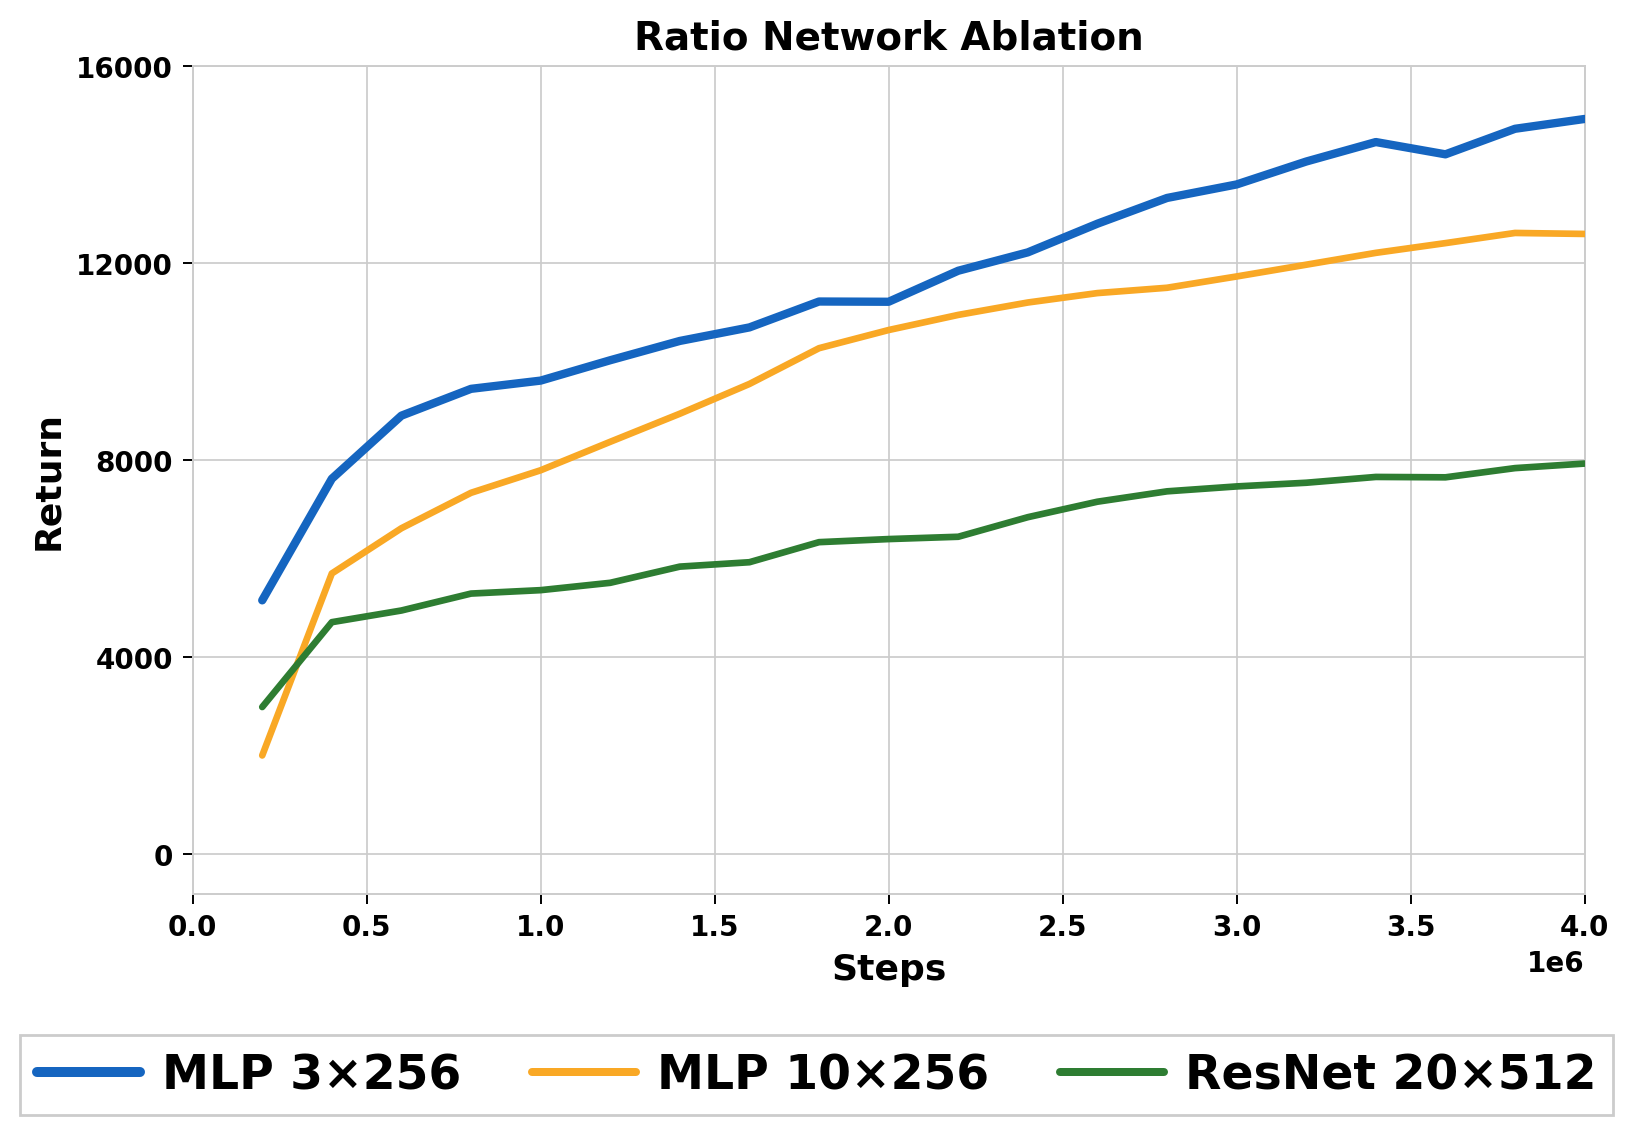
\includegraphics[width=\linewidth]{halfcheetah_ratio_ablation_red.png}
        \caption{\small Effect of ratio network architecture.}
    \end{subfigure}
    \hfill
    \begin{subfigure}{0.49\linewidth}
        \centering
        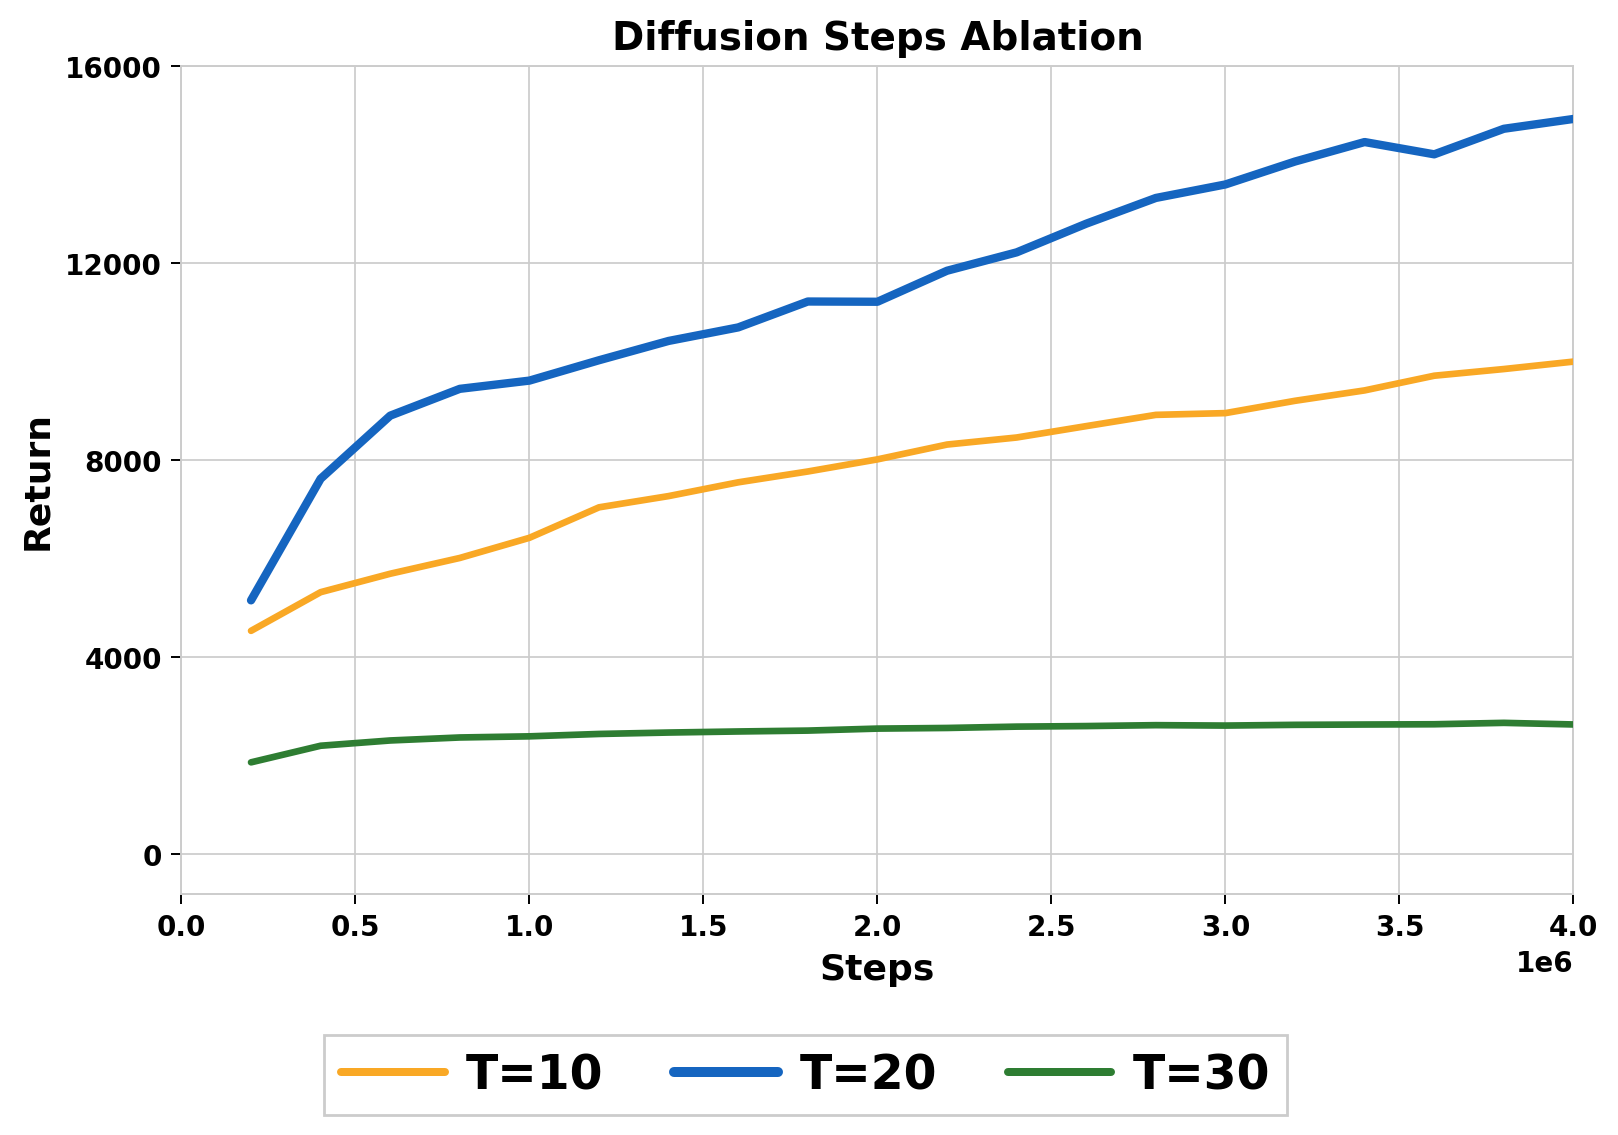
\includegraphics[width=\linewidth]{halfcheetah_diffusion_steps_ablation_red.png}
        \caption{\small Effect of the number of diffusion steps.}
    \end{subfigure}

    \vspace{-2mm}
    \caption{{\small Ablation study of DoobPPO on OpenAI Gym MuJoCo \texttt{HalfCheetah-v4}.
    \textbf{(a)} Effect of the ratio network architecture on policy performance.
    \textbf{(b)} Different diffusion steps lead to significantly different performance, with moderate steps performing best.}}
    \label{fig:ablation_two}
\end{figure}

\subsection{Diffusion Policy.}

\paragraph{Ablation Study on Ratio Network Size.}
We study the sensitivity of DoobPPO to the ratio-network architecture on \texttt{HalfCheetah-v4}.
We compare three variants: an MLP ratio network with 3 layers of width 256, a deeper MLP with 10 layers of width 256, and a larger ResNet-style architecture with 20 layers of width 512.
As shown in Figure~\ref{fig:ablation_two}, the simple 3$\times$256 MLP achieves the best performance, consistently outperforming both the deeper MLP and the larger ResNet-style model.
This suggests that increasing the capacity of the ratio network does not necessarily improve performance, and may even make optimization less effective.
Based on this result, we use the 3$\times$256 MLP ratio network in all diffusion-policy experiments.

\paragraph{Ablation Study on Diffusion Steps.}
We also study the sensitivity of DoobPPO to the number of diffusion steps on \texttt{HalfCheetah-v4}.
We compare three settings, namely $T=10$, $T=20$, and $T=30$.
The results show that $T=20$ achieves the best overall performance, while $T=10$ remains competitive but consistently underperforms $T=20$, and $T=30$ leads to a substantial degradation.
These results suggest that DoobPO benefits from a moderately sized diffusion process rather than a very shallow or overly long denoising chain.
Therefore, we use $20$ diffusion steps in all diffusion-policy experiments.

\subsection{Flow Policy.}

\begin{figure}[h]
    \centering
    \begin{subfigure}{0.49\linewidth}
        \centering
        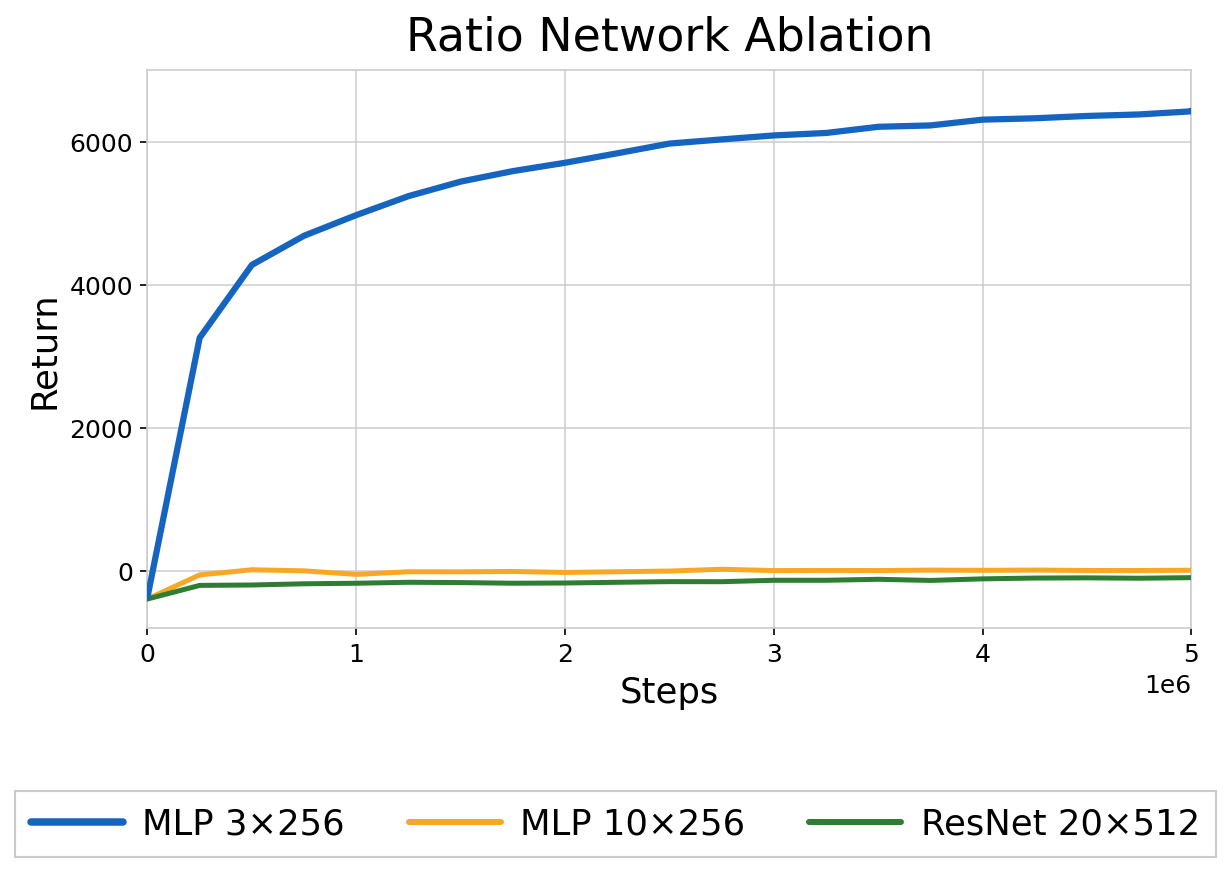
\includegraphics[width=\linewidth]{halfcheetah_flow_ratio_ablation_red.png}
        \caption{\small Effect of ratio network architecture.}
    \end{subfigure}
    \hfill
    \begin{subfigure}{0.49\linewidth}
        \centering
        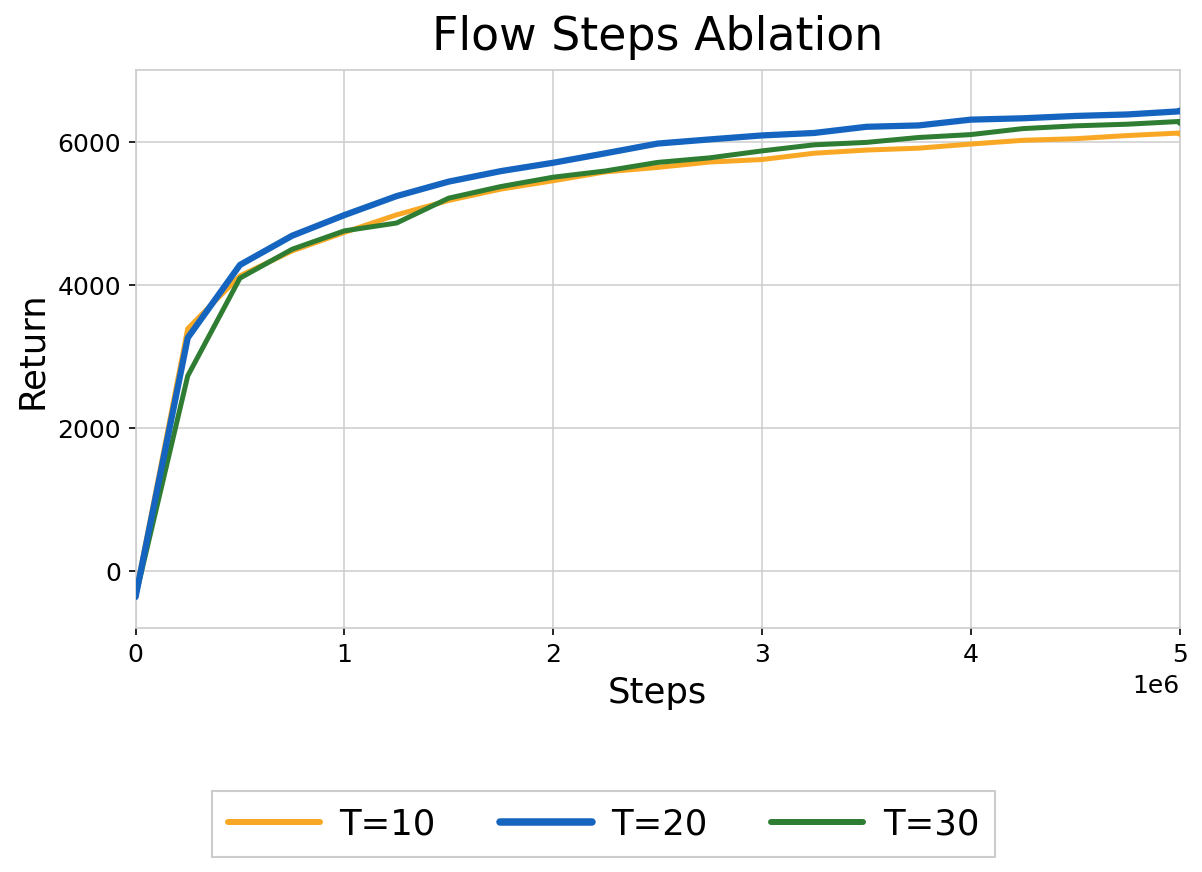
\includegraphics[width=\linewidth]{halfcheetah_flow_steps_ablation_red.png}
        \caption{\small Effect of the number of flow steps.}
    \end{subfigure}

    \vspace{-2mm}
    \caption{{\small Ablation study of DoobGRPO flow policy on OpenAI Gym MuJoCo \texttt{HalfCheetah-v4}.
    \textbf{(a)} Only the lightweight MLP 3$\times$256 ratio network learns effectively, while deeper and larger architectures fail to train.
    \textbf{(b)} Performance is robust to the number of flow steps, with $T{=}20$ achieving the best result and $T{=}10$, $T{=}30$ remaining competitive.}}
    \label{fig:ablation_flow}
\end{figure}

\paragraph{Ablation Study on Ratio Network Size.}
We study the sensitivity of DoobGRPO to the ratio-network architecture on \texttt{HalfCheetah-v4} with flow policies.
We compare the same three variants as in the diffusion-policy setting: an MLP ratio network with 3 layers of width 256, a deeper MLP with 10 layers of width 256, and a ResNet-style architecture with 20 blocks of width 512.
As shown in Figure~\ref{fig:ablation_flow}(a), the simple 3$\times$256 MLP achieves the best performance with a peak return of 6433, while both the deeper MLP (peak return 23) and the larger ResNet (peak return $-$94) fail to learn meaningful policies.
This is consistent with the diffusion-policy ablation, confirming that a lightweight ratio network is critical for stable training across both generative-model backbones.

\paragraph{Ablation Study on Flow Steps.}
We also study the sensitivity of DoobGRPO to the number of flow integration steps on \texttt{HalfCheetah-v4}.
We compare $T=10$, $T=20$, and $T=30$.
As shown in Figure~\ref{fig:ablation_flow}(b), the default setting $T=20$ achieves the best peak performance (6433), while $T=10$ (6120) and $T=30$ (6282) remain competitive but slightly underperform $T=20$.
These results suggest that DoobPO is relatively robust to the choice of flow steps, with $T=20$ providing the best trade-off between sampling quality and computational cost.
We use $20$ flow steps in all flow-policy experiments.


\clearpage
\section{Algorithms}

\subsection{Diffusion Policy Optimization with DoobPO}

\begin{algorithm}[h]
\caption{Diffusion Policy Optimization with DoobPO}
\label{alg:rwdm_ppo}
\begin{algorithmic}[1]
\Require Environment MDP $\mathcal{M}=(\mathcal{S},\mathcal{A},P,R,\gamma)$;
pre-trained score model $g_{\phi}$;
reinforcement learning objective $J_{\mathrm{RL}}$;
advantage estimator $\hat{A}$;
ratio network $r_\beta$;
ratio regularization coefficient $\lambda_{\mathrm{reg}}$;
iteration $K$
\State \textbf{Initialize:} drift model $\theta_1=\phi$; ratio net $\beta_1$.
\For{$k=1,2,\ldots,K$}
    \State Add rollout samples to replay buffer $\mathcal{D}$ from $\mathcal{M}$ using current policy $\pi^k$ induced by $g_{\theta_k}$
    \State Estimate advantage of current policy $A^{\pi^k}\leftarrow \hat{A}(\mathcal{D})$

    \State \textbf{Ratio learning update}
    \State Update $\beta$ by optimizing the regularized reinforcement learning objective
    \begin{align*}
        \beta_{k+1}
        \leftarrow
        \argmax_{\beta}
        \Big\{
        J_{\mathrm{RL}}(\beta)
        -
        \lambda_{\mathrm{reg}}
        \E_{o\sim\mathcal D}
        \Big[
        \big(
        \E_{a\sim \pi^k(\cdot|o)}[r_\beta(o,a)]-1
        \big)^2
        \Big]
        \Big\}.
    \end{align*}

    \State \textbf{Doob's drift matching update}
    \State For each $(o,a)\in\mathcal{D}$, sample $t\sim U[0,T]$ and generate noised action $x_t$
    \begin{align*}
        x_t \leftarrow \sqrt{\bar\alpha_t}\,a
    + \sqrt{1-\bar\alpha_t}\,z,
\quad z\sim\mathcal N(0,I)
    \end{align*}
    \State Update $\theta$ by minimizing the conditional drift matching objective
    \begin{align*}
        \theta_{k+1}\leftarrow \argmin_{\theta}
        \E_{(o,a,x_t,t)\sim\mathcal{D}}
        \Big[
        r_{\beta_{k+1}}(o,a)
        \Big\|
        -\frac{x_t-\sqrt{\bar\alpha_t}\,a}
    {1-\bar\alpha_t}
    -g_\theta(x_t,t,o)
        \Big\|_2^2
        \Big]
    \end{align*}
\EndFor
\State \textbf{Output:} Policy $\pi^{K+1}$ with learned drift $g_{\theta_{K+1}}$
\end{algorithmic}
\end{algorithm}


\clearpage
\subsection{Flow Policy Optimization with DoobPO}

\begin{algorithm}[h]
\caption{Flow Policy Optimization with DoobPO}
\label{alg:rwdm_ppo_fm}
\begin{algorithmic}[1]
\Require Environment MDP $\mathcal{M}=(\mathcal{S},\mathcal{A},P,R,\gamma)$;
pre-trained velocity model $u_{\phi}$;
reinforcement learning objective $J_{\mathrm{RL}}$;
advantage estimator $\hat{A}$;
ratio network $r_\beta$;
ratio regularization coefficient $\lambda_{\mathrm{reg}}$;
iteration $K$
\State \textbf{Initialize:} velocity model $\theta_1=\phi$; ratio net $\beta_1$.
\For{$k=1,2,\ldots,K$}
    \State Add rollout samples to replay buffer $\mathcal{D}$ from $\mathcal{M}$ using current policy $\pi^k$ induced by $u_{\theta_k}$
    \State Estimate advantage of current policy $A^{\pi^k}\leftarrow \hat{A}(\mathcal{D})$

    \State \textbf{Ratio learning update}
    \State Update $\beta$ by optimizing the regularized reinforcement learning objective
    \begin{align*}
        \beta_{k+1}
        \leftarrow
        \argmax_{\beta}
        \Big\{
        J_{\mathrm{RL}}(\beta)
        -
        \lambda_{\mathrm{reg}}
        \E_{o\sim\mathcal D}
        \Big[
        \big(
        \E_{a\sim \pi^k(\cdot|o)}[r_\beta(o,a)]-1
        \big)^2
        \Big]
        \Big\}.
    \end{align*}

    \State \textbf{Drift matching update}
    \State For each $(o,a)\in\mathcal{D}$, sample $t \sim U[0,T]$ and generate intermediate action $x_t$ by
    \begin{align*}
        x_t \leftarrow \alpha_t z
        + \beta_t a,
        \quad z \sim N(0,I)
    \end{align*}
    \State Update $\theta$ by minimizing the conditional drift matching objective
    \begin{align*}
        \theta_{k+1} \leftarrow \argmin_{\theta}
        \E_{(o,a,x_t,t)\sim \mathcal{D}}
        \Big[ r_{\beta_{k+1}}(o,a)\,
        \|
            \dot{\alpha}_t z + \dot{\beta}_t a
            - u_\theta(x_t,t,o)
        \|_2^2
        \Big]
    \end{align*}
\EndFor
\State \textbf{Output:} Policy $\pi^{K+1}$ with learned velocity $u_{\theta_{K+1}}$
\end{algorithmic}
\end{algorithm}
